\section{Experiment 2}\label{sec:experiment_2}
This section will describe the second experiment of the project. The second experiment covers how many dimensions are necessary to still have a good accuracy of arround 95\%\todo{lower this to something more resonable}. The experiment will only be done on 15.000 samples, instead of the entire data set of 60.000 samples, due to issues regarding memory usage. The experimant will focus on when different dimensionality reduction methods, show a noticable drop in accuracy due to too few dimensions. 


\subsection{Rules and evaluation of the experiment}\label{subsec:experiment_2_rules}
This section will cover the rules of the second experiment, and also how the results of the experiment will be evaluated.

The second experiment is done on a subset of the entire data set. With 15.000 samples in the training set, and the usual 10.000 samples in the test set. Instead of the standard 60.000 samples in the training set and 10.000 in the test set.\todo{Remember to discuss why only a limited amount of the data set and give detailed reasons and difficulties}

The values from the \gls{mnist} dataset will be normalized using standard scalar, for each of the dimensionality reduction methods. This is to ensure that the values are on the same scale, so that the results are not skewed by different scales.\todo{Discussion?}

There will be done hyperparamater tuning, using gridsearch, on each of the dimensionality reduction methods. This is to ensure that good hyperparamaters are found for each number of components, so that the results are not sqewed by hyperparamaters that are not optimal for the number of components. If it was chosen to use fixed value for the hyperparamaters, the results could be skewed for some certain number of components.\todo{Discussion?}

The dimensionality reduction methods that will be used are \gls{pca}, \gls{lda}, \gls{isomap} and \gls{kpca}. The number of components will be varied from 2 to 50.\todo{Remember to discuss why this range} \gls{lda} is an exception, as the maximum number of components is the number of classes, which is 10 for the \gls{mnist} dataset.\todo{Ensure it is 10 and not 9} Meaning that the range of components for \gls{lda} will be from 2-10.

The values that will be used to evaluate this experiment, are the \texttt{mean\_fit\_time} to evaluate the time it takes to fit the model, the \texttt{mean\_test\_score} based on \texttt{param\_pca\_\_n\_components} to evaluate the accuracy of the modele with the number of components used.

With the results from running the experiment, a plot will be made to show the accuracy of the models with the number of components used. The plot is used to visually represent when the accuracy starts to drop. 


\subsection{Results}\label{subsec:experiment_2_results}
This section will cover the results gathered from running the second experiment. Each of the dimensionality reduction methods will be presented using scatter plots. The scatter plots will show the number of components used along the x-axis, and the accuracy of the model along the y-axis. The results will then be compared, and evaluated based on the rules of the experiment. The main focus of the evaluation will be on when the accuracy starts to noticablly drop, and how many components are needed to still have a good accuracy. The scatter plots are used to visiually represent the results, and to make it easier to see when the accuracy starts to drop. But the specific values of the accuracy will also be discussed, these values are taken from the csv\todo{add csv to gls} files generated from running the second experiment. \todo{Also add explanation to multiple dots on the same x-value}

\subsubsection{\gls{pca}}\label{subsubsec:experiment_2_pca}
\gls{pca} is a linear dimensionality reduction method, the scatter plot representing this method can be seen in \autoref{fig:experiment_2_pca_svm}. Ofcourse as one would expect, the accuracy of the model increases as the number of components increases. But arround 20 components, the accuracy starts to drop, the accuracy has a noticable drop between 10 and 20 components, and the accuracy has a drastic drop for each component removed below 10 components. This is to be expected as the lower the number of components the model has to work with, the more information is lost, and the gain of each added component decreases as the number of components increases. With all 50 components the accuracy of the model is ~91.9\% and first really only drop below 91\% arround 43 components. With \gls{pca} there are multiple dots for each component, so the accuracy varies slightly depending on the hyperparamaters used, but the general trend is the same.

A noticable drop can especially be seen arround 20 components, where the accuracy starts dropping 

\begin{figure}[htb!]
    \centering
    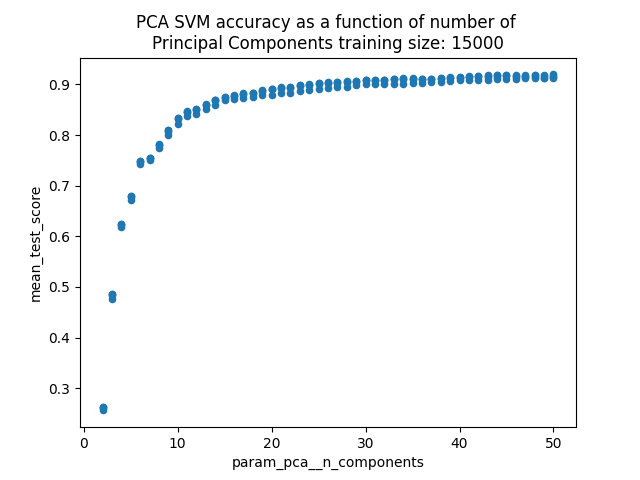
\includegraphics[scale=0.5]{figures/experiment_two/pca_svm_15000.png}
    \caption{Accuracy of the SVM model with PCA as dimensionality reduction method, with the number of components used.}
    \label{fig:experiment_2_pca_svm}
\end{figure}

\subsubsection{\gls{lda}}\label{subsubsec:experiment_2_lda}

\subsection{Discussion}\label{subsec:experiment_2_discussion}



% intro
% presentation af de experimenter vi har valgt og hvorfor vi har valgt dem?
% experiment 1 exemple
%     detaljeret gennemgang af regler og evaluering
%     fremvisning af resultater
%     opsumering af resultater
%     diskussion af resultater og hvad der ellers var spændende evaluering af hvorfor det blev sådan.